\section{一个有趣的应用:彩虹表}\label{sec:18-7}

令 $h:\mathcal{P}\to\mathcal{Y}$ 是一个随机函数,并设置 $N:=|\mathcal{P}|$。我们来看看计算 $h$ 的逆这个一般的问题。我们假设 $|\mathcal{Y}|\geq N$,因为这是实践中的典型情况。比如说,$\mathcal{P}$ 可能是所有 $8$ 字符口令的集合,而 $\mathcal{Y}=\{0,1\}^{256}$。

令 $pw\overset{\rm R}\leftarrow\mathcal{P}$,并令 $y\leftarrow h(pw)$。显然,对 $\mathcal{P}$ 的所有可能性进行穷举搜索,只要对 $h$ 进行最多 $N$ 次查询,就可以确保找到 $y$ 的原像。在本节中,我们将开发一种更快的算法,它使用一种称作\textbf{彩虹表(rainbow table)}的方法来求取 $h$ 的逆。求逆算法 $\mathcal{A}=(\mathcal{A}_0,\mathcal{A}_1)$ 分两个阶段进行:
\begin{itemize}
	\item 预处理阶段:算法 $\mathcal{A}_0$ 查询 $h$,并输出一张包含 $\ell$ 个 $\mathcal{P}^2$ 中的数对的表 $L$,其中 $\ell$ 是某个正整数。该预处理阶段耗时为 $O(N)$,但它在获知挑战 $y$ 之前已被离线完成。产生的表 $L$ 被称为彩虹表,它必须被妥善储存,以便在第二阶段使用。
	\item 攻击阶段:一旦被赋予一个挑战 $y\in\mathcal{Y}$,$\mathcal{A}_1$ 算法就会以 $\mathcal{A}_1(L,y)$ 的方式被调用,使用 $L$ 快速地找到 $y$ 的逆元。它能以接近 $1$ 的概率输出一个 $h^{-1}(y)$ 中的原像 $pw'$。
\end{itemize}
令 $t$ 为 $\mathcal{A}_1$ 在攻击阶段中的运行时间。下面,我们展示如何在时间 $t$ 内计算 $h$ 的逆,其中:
\begin{equation}\label{eq:18-9}
t\times\ell^2\approx N^2
\end{equation}
举例来说,如果我们可以存储一个大小为 $\ell=N^{2/3}$ 的表 $L$,我们就可以在 $t\approx N^{2/3}$ 的时间内以接近 $1$ 的概率计算 $h$ 的逆,这比在 $\mathcal{P}$ 上进行穷举搜索要快得多。

式 \ref{eq:18-9} 被称作\textbf{时空权衡(time-space tradeoff)}。我们留给表 $L$ 的空间越大,求取 $h$ 的逆的速度就越快。当然,一旦我们有了表 $L$,我们就可以用它来快速地找到许多 $\mathcal{Y}$ 中元素的逆。

正如 \ref{subsubsec:18-3-1-3} 小节所述,彩虹表通常被用于破解未加盐的口令。它们也可以用于从已知的明文-密文对 $\big(m,\,c=E(k,m)\big)$ 中恢复分组密码 $(E,D)$ 的秘钥 $k$。这是因为密钥 $k$ 就是函数 $h(k):=E(k,m)$ 在 $c$ 点处的逆元。如果 $m$ 足够长,或者提供足够多的明文-密文对,那么这个逆元 $k$ 就是唯一的。将此结论应用于 AES-128,我们就可以得到一个大小为 $128\times(2^{128})^{(2/3)}\approx 128\times 2^{85}$ 比特的表 $L$(约 $10$ 亿艾字节),它可以被用来在 $2^{85}$ 的时间内破解 AES。它的耗时在今天来看可能太长,但在几十年后可能会变得可以接受。我们曾在第 \ref{subsubsec:4-2-2-1} 小节中讨论过这种威胁。这种威胁也是迫使人们转向 AES-256 的一个很重要的原因。但是请注意,建立表 $L$ 需要大量(一次性的)工作,即大约 $2^{128}$ 次对 AES-128 的评估。

细心的读者会注意到,式 \ref{eq:18-9} 中的边界在 $\ell=1$ 时相当差,此时,我们有 $t\approx N^2$。这比耗时为 $N$ 的简单穷举搜索还要差得多。这说明,彩虹表算法对于某些 $\ell$ 值来说并不严格。改进时空权衡 \ref{eq:18-9} 是一个长期存在的开放性问题(见练习 \ref{exer:18-7})。

\begin{snote}[Hellman 的基本时空权衡。]
第一个用于求取随机函数的逆的时空权衡是由 Hellman 发明的,它是对 DES 的短密钥设计($56$ 比特)的一个有力批评。Hellman 的方法使用了一个可有效计算的辅助函数 $g:\mathcal{Y}\to\mathcal{P}$,被称为\textbf{还原函数(reduction function)}。它能将 $h$ 的一个 $\mathcal{Y}$ 上的输出``还原"为一个 $\mathcal{P}$ 上的元素。简单起见,我们假设 $g$ 也是一个随机函数。那么,函数 $f(pw):=g(h(pw))$ 就会将 $\mathcal{P}$ 映射到它自身。

预处理算法 $\mathcal{A}_0$ 使用函数 $f:\mathcal{P}\to\mathcal{P}$,它以两个正常数 $\tau$ 和 $\ell$ 为参数。回顾一下,对于 $\tau>0$,函数 $f^{(\tau)}$ 就是定义在 \ref{eq:18-5} 中的 $f$ 的 $\tau$ 次迭代。图 \ref{fig:18-13-a} 直观地展示了算法 $\mathcal{A}_0$ 的工作原理,它运行如下:

\vspace*{10pt}

\hspace*{5pt} 算法 $\mathcal{A}_0$:(预处理 $h$)\\
\hspace*{50pt} 对于 $i=1,\dots,\ell$:\\
\hspace*{75pt} 随机选取 $pw_i\overset{\rm R}\leftarrow\mathcal{P}$\\
\hspace*{75pt} 令 $z_i\leftarrow f^{(\tau)}(pw_i)\in\mathcal{P}$
\hspace*{100pt} // \emph{对 $f$ 进行 $\tau$ 次评估}

\vspace*{5pt}

\hspace*{28.5pt} 输出 $L:=\big\{(pw_1,z_1),\dots,(pw_\ell,z_\ell)\big\}\subseteq\mathcal{P}^2$
\hspace*{37pt} // \emph{输出 $\ell$ 个 $\mathcal{P}^2$ 中的数对}

\vspace*{10pt}

\begin{figure}
  \centering
  \subfigure[Hellman 的基本时空权衡]{
  	  \tikzset{every picture/.style={line width=0.75pt}}

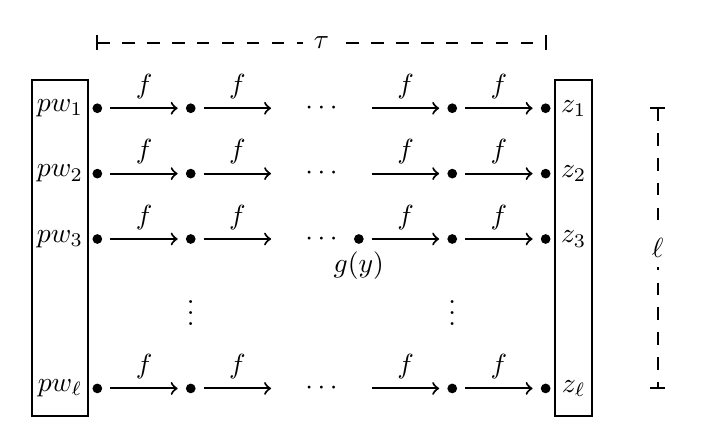
\begin{tikzpicture}[x=0.75pt,y=0.75pt,yscale=-0.9,xscale=0.9]

\draw   (40,40) -- (70,40) -- (70,220) -- (40,220) -- cycle ;
\draw   (320,40) -- (340,40) -- (340,220) -- (320,220) -- cycle ;

\draw  [fill={rgb, 255:red, 0; green, 0; blue, 0 }  ,fill opacity=1 ] (73,55) .. controls (73,53.9) and (73.9,53) .. (75,53) .. controls (76.1,53) and (77,53.9) .. (77,55) .. controls (77,56.1) and (76.1,57) .. (75,57) .. controls (73.9,57) and (73,56.1) .. (73,55) -- cycle ;
\draw  [fill={rgb, 255:red, 0; green, 0; blue, 0 }  ,fill opacity=1 ] (73,90) .. controls (73,88.9) and (73.9,88) .. (75,88) .. controls (76.1,88) and (77,88.9) .. (77,90) .. controls (77,91.1) and (76.1,92) .. (75,92) .. controls (73.9,92) and (73,91.1) .. (73,90) -- cycle ;
\draw  [fill={rgb, 255:red, 0; green, 0; blue, 0 }  ,fill opacity=1 ] (73,125) .. controls (73,123.9) and (73.9,123) .. (75,123) .. controls (76.1,123) and (77,123.9) .. (77,125) .. controls (77,126.1) and (76.1,127) .. (75,127) .. controls (73.9,127) and (73,126.1) .. (73,125) -- cycle ;
\draw  [fill={rgb, 255:red, 0; green, 0; blue, 0 }  ,fill opacity=1 ] (73,205) .. controls (73,203.9) and (73.9,203) .. (75,203) .. controls (76.1,203) and (77,203.9) .. (77,205) .. controls (77,206.1) and (76.1,207) .. (75,207) .. controls (73.9,207) and (73,206.1) .. (73,205) -- cycle ;
\draw  [fill={rgb, 255:red, 0; green, 0; blue, 0 }  ,fill opacity=1 ] (123,55) .. controls (123,53.9) and (123.9,53) .. (125,53) .. controls (126.1,53) and (127,53.9) .. (127,55) .. controls (127,56.1) and (126.1,57) .. (125,57) .. controls (123.9,57) and (123,56.1) .. (123,55) -- cycle ;
\draw  [fill={rgb, 255:red, 0; green, 0; blue, 0 }  ,fill opacity=1 ] (263,55) .. controls (263,53.9) and (263.9,53) .. (265,53) .. controls (266.1,53) and (267,53.9) .. (267,55) .. controls (267,56.1) and (266.1,57) .. (265,57) .. controls (263.9,57) and (263,56.1) .. (263,55) -- cycle ;
\draw  [fill={rgb, 255:red, 0; green, 0; blue, 0 }  ,fill opacity=1 ] (313,55) .. controls (313,53.9) and (313.9,53) .. (315,53) .. controls (316.1,53) and (317,53.9) .. (317,55) .. controls (317,56.1) and (316.1,57) .. (315,57) .. controls (313.9,57) and (313,56.1) .. (313,55) -- cycle ;
\draw  [fill={rgb, 255:red, 0; green, 0; blue, 0 }  ,fill opacity=1 ] (123,90) .. controls (123,88.9) and (123.9,88) .. (125,88) .. controls (126.1,88) and (127,88.9) .. (127,90) .. controls (127,91.1) and (126.1,92) .. (125,92) .. controls (123.9,92) and (123,91.1) .. (123,90) -- cycle ;
\draw  [fill={rgb, 255:red, 0; green, 0; blue, 0 }  ,fill opacity=1 ] (263,90) .. controls (263,88.9) and (263.9,88) .. (265,88) .. controls (266.1,88) and (267,88.9) .. (267,90) .. controls (267,91.1) and (266.1,92) .. (265,92) .. controls (263.9,92) and (263,91.1) .. (263,90) -- cycle ;
\draw  [fill={rgb, 255:red, 0; green, 0; blue, 0 }  ,fill opacity=1 ] (313,90) .. controls (313,88.9) and (313.9,88) .. (315,88) .. controls (316.1,88) and (317,88.9) .. (317,90) .. controls (317,91.1) and (316.1,92) .. (315,92) .. controls (313.9,92) and (313,91.1) .. (313,90) -- cycle ;
\draw  [fill={rgb, 255:red, 0; green, 0; blue, 0 }  ,fill opacity=1 ] (123,125) .. controls (123,123.9) and (123.9,123) .. (125,123) .. controls (126.1,123) and (127,123.9) .. (127,125) .. controls (127,126.1) and (126.1,127) .. (125,127) .. controls (123.9,127) and (123,126.1) .. (123,125) -- cycle ;
\draw  [fill={rgb, 255:red, 0; green, 0; blue, 0 }  ,fill opacity=1 ] (263,125) .. controls (263,123.9) and (263.9,123) .. (265,123) .. controls (266.1,123) and (267,123.9) .. (267,125) .. controls (267,126.1) and (266.1,127) .. (265,127) .. controls (263.9,127) and (263,126.1) .. (263,125) -- cycle ;
\draw  [fill={rgb, 255:red, 0; green, 0; blue, 0 }  ,fill opacity=1 ] (313,125) .. controls (313,123.9) and (313.9,123) .. (315,123) .. controls (316.1,123) and (317,123.9) .. (317,125) .. controls (317,126.1) and (316.1,127) .. (315,127) .. controls (313.9,127) and (313,126.1) .. (313,125) -- cycle ;
\draw  [fill={rgb, 255:red, 0; green, 0; blue, 0 }  ,fill opacity=1 ] (123,205) .. controls (123,203.9) and (123.9,203) .. (125,203) .. controls (126.1,203) and (127,203.9) .. (127,205) .. controls (127,206.1) and (126.1,207) .. (125,207) .. controls (123.9,207) and (123,206.1) .. (123,205) -- cycle ;
\draw  [fill={rgb, 255:red, 0; green, 0; blue, 0 }  ,fill opacity=1 ] (263,205) .. controls (263,203.9) and (263.9,203) .. (265,203) .. controls (266.1,203) and (267,203.9) .. (267,205) .. controls (267,206.1) and (266.1,207) .. (265,207) .. controls (263.9,207) and (263,206.1) .. (263,205) -- cycle ;
\draw  [fill={rgb, 255:red, 0; green, 0; blue, 0 }  ,fill opacity=1 ] (313,205) .. controls (313,203.9) and (313.9,203) .. (315,203) .. controls (316.1,203) and (317,203.9) .. (317,205) .. controls (317,206.1) and (316.1,207) .. (315,207) .. controls (313.9,207) and (313,206.1) .. (313,205) -- cycle ;
\draw  [fill={rgb, 255:red, 0; green, 0; blue, 0 }  ,fill opacity=1 ] (213,125) .. controls (213,123.9) and (213.9,123) .. (215,123) .. controls (216.1,123) and (217,123.9) .. (217,125) .. controls (217,126.1) and (216.1,127) .. (215,127) .. controls (213.9,127) and (213,126.1) .. (213,125) -- cycle ;

\draw  [->]  (82,55) -- (118,55) ;
\draw  [->]  (132,55) -- (168,55) ;
\draw  [->]  (222,55) -- (258,55) ;
\draw  [->]  (272,55) -- (308,55) ;

\draw  [->]  (82,90) -- (118,90) ;
\draw  [->]  (132,90) -- (168,90) ;
\draw  [->]  (222,90) -- (258,90) ;
\draw  [->]  (272,90) -- (308,90) ;

\draw  [->]  (82,125) -- (118,125) ;
\draw  [->]  (132,125) -- (168,125) ;
\draw  [->]  (222,125) -- (258,125) ;
\draw  [->]  (272,125) -- (308,125) ;

\draw  [->]  (82,205) -- (118,205) ;
\draw  [->]  (132,205) -- (168,205) ;
\draw  [->]  (222,205) -- (258,205) ;
\draw  [->]  (272,205) -- (308,205) ;


\draw  [dash pattern={on 4.5pt off 4.5pt}]  (75,20) -- (315,20) ;
\draw [shift={(315,20)}, rotate = 180]  (0,4) -- (0,-4)   ;
\draw [shift={(75,20)}, rotate = 180]   (0,4) -- (0,-4)   ;

\draw  [dash pattern={on 4.5pt off 4.5pt}]  (375,55) -- (375,205) ;
\draw [shift={(375,205)}, rotate = 270] (0,4) -- (0,-4)   ;
\draw [shift={(375,55)}, rotate = 270]  (0,4) -- (0,-4)   ;

\draw  [draw opacity=0][fill={rgb, 255:red, 255; green, 255; blue, 255 }  ,fill opacity=1 ] (185,15) -- (205,15) -- (205,25) -- (185,25) -- cycle ;
\draw  [draw opacity=0][fill={rgb, 255:red, 255; green, 255; blue, 255 }  ,fill opacity=1 ] (370,120) -- (380,120) -- (380,140) -- (370,140) -- cycle ;


\draw (55,55) node    {$pw_{1}$};
\draw (55,90) node    {$pw_{2}$};
\draw (55,125) node    {$pw_{3}$};
\draw (55,205) node    {$pw_{\ell }$};
\draw (195,55) node    {$\cdots $};
\draw (195,90) node    {$\cdots $};
\draw (195,125) node    {$\cdots $};
\draw (195,205) node    {$\cdots $};
\draw (330,55) node    {$z_{1}$};
\draw (330,90) node    {$z_{2}$};
\draw (330,125) node    {$z_{3}$};
\draw (330,205) node    {$z_{\ell }$};
\draw (125,160.03) node    {$\vdots $};
\draw (265,160.03) node    {$\vdots $};
\draw (100,51.6) node [anchor=south] [inner sep=0.75pt]    {$f$};
\draw (150,51.6) node [anchor=south] [inner sep=0.75pt]    {$f$};
\draw (240,51.6) node [anchor=south] [inner sep=0.75pt]    {$f$};
\draw (290,51.6) node [anchor=south] [inner sep=0.75pt]    {$f$};
\draw (100,86.6) node [anchor=south] [inner sep=0.75pt]    {$f$};
\draw (150,86.6) node [anchor=south] [inner sep=0.75pt]    {$f$};
\draw (240,86.6) node [anchor=south] [inner sep=0.75pt]    {$f$};
\draw (290,86.6) node [anchor=south] [inner sep=0.75pt]    {$f$};
\draw (100,121.6) node [anchor=south] [inner sep=0.75pt]    {$f$};
\draw (150,121.6) node [anchor=south] [inner sep=0.75pt]    {$f$};
\draw (240,121.6) node [anchor=south] [inner sep=0.75pt]    {$f$};
\draw (290,121.6) node [anchor=south] [inner sep=0.75pt]    {$f$};
\draw (100,201.6) node [anchor=south] [inner sep=0.75pt]    {$f$};
\draw (150,201.6) node [anchor=south] [inner sep=0.75pt]    {$f$};
\draw (240,201.6) node [anchor=south] [inner sep=0.75pt]    {$f$};
\draw (290,201.6) node [anchor=south] [inner sep=0.75pt]    {$f$};
\draw (215,130.4) node [anchor=north] [inner sep=0.75pt]    {$g(y)$};
\draw (195,20) node    {$\tau$};
\draw (375,130) node    {$\ell$};

\end{tikzpicture}
  	  \label{fig:18-13-a}
  }
  \subfigure[彩虹表]{
      \tikzset{every picture/.style={line width=0.75pt}}

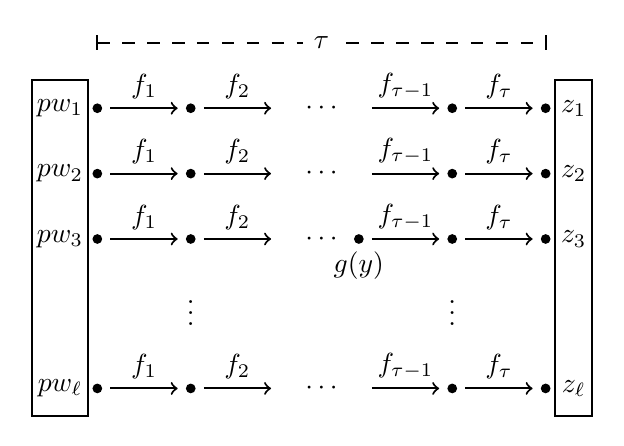
\begin{tikzpicture}[x=0.75pt,y=0.75pt,yscale=-0.9,xscale=0.9]

\draw   (40,40) -- (70,40) -- (70,220) -- (40,220) -- cycle ;
\draw   (320,40) -- (340,40) -- (340,220) -- (320,220) -- cycle ;

\draw  [fill={rgb, 255:red, 0; green, 0; blue, 0 }  ,fill opacity=1 ] (73,55) .. controls (73,53.9) and (73.9,53) .. (75,53) .. controls (76.1,53) and (77,53.9) .. (77,55) .. controls (77,56.1) and (76.1,57) .. (75,57) .. controls (73.9,57) and (73,56.1) .. (73,55) -- cycle ;
\draw  [fill={rgb, 255:red, 0; green, 0; blue, 0 }  ,fill opacity=1 ] (73,90) .. controls (73,88.9) and (73.9,88) .. (75,88) .. controls (76.1,88) and (77,88.9) .. (77,90) .. controls (77,91.1) and (76.1,92) .. (75,92) .. controls (73.9,92) and (73,91.1) .. (73,90) -- cycle ;
\draw  [fill={rgb, 255:red, 0; green, 0; blue, 0 }  ,fill opacity=1 ] (73,125) .. controls (73,123.9) and (73.9,123) .. (75,123) .. controls (76.1,123) and (77,123.9) .. (77,125) .. controls (77,126.1) and (76.1,127) .. (75,127) .. controls (73.9,127) and (73,126.1) .. (73,125) -- cycle ;
\draw  [fill={rgb, 255:red, 0; green, 0; blue, 0 }  ,fill opacity=1 ] (73,205) .. controls (73,203.9) and (73.9,203) .. (75,203) .. controls (76.1,203) and (77,203.9) .. (77,205) .. controls (77,206.1) and (76.1,207) .. (75,207) .. controls (73.9,207) and (73,206.1) .. (73,205) -- cycle ;
\draw  [fill={rgb, 255:red, 0; green, 0; blue, 0 }  ,fill opacity=1 ] (123,55) .. controls (123,53.9) and (123.9,53) .. (125,53) .. controls (126.1,53) and (127,53.9) .. (127,55) .. controls (127,56.1) and (126.1,57) .. (125,57) .. controls (123.9,57) and (123,56.1) .. (123,55) -- cycle ;
\draw  [fill={rgb, 255:red, 0; green, 0; blue, 0 }  ,fill opacity=1 ] (263,55) .. controls (263,53.9) and (263.9,53) .. (265,53) .. controls (266.1,53) and (267,53.9) .. (267,55) .. controls (267,56.1) and (266.1,57) .. (265,57) .. controls (263.9,57) and (263,56.1) .. (263,55) -- cycle ;
\draw  [fill={rgb, 255:red, 0; green, 0; blue, 0 }  ,fill opacity=1 ] (313,55) .. controls (313,53.9) and (313.9,53) .. (315,53) .. controls (316.1,53) and (317,53.9) .. (317,55) .. controls (317,56.1) and (316.1,57) .. (315,57) .. controls (313.9,57) and (313,56.1) .. (313,55) -- cycle ;
\draw  [fill={rgb, 255:red, 0; green, 0; blue, 0 }  ,fill opacity=1 ] (123,90) .. controls (123,88.9) and (123.9,88) .. (125,88) .. controls (126.1,88) and (127,88.9) .. (127,90) .. controls (127,91.1) and (126.1,92) .. (125,92) .. controls (123.9,92) and (123,91.1) .. (123,90) -- cycle ;
\draw  [fill={rgb, 255:red, 0; green, 0; blue, 0 }  ,fill opacity=1 ] (263,90) .. controls (263,88.9) and (263.9,88) .. (265,88) .. controls (266.1,88) and (267,88.9) .. (267,90) .. controls (267,91.1) and (266.1,92) .. (265,92) .. controls (263.9,92) and (263,91.1) .. (263,90) -- cycle ;
\draw  [fill={rgb, 255:red, 0; green, 0; blue, 0 }  ,fill opacity=1 ] (313,90) .. controls (313,88.9) and (313.9,88) .. (315,88) .. controls (316.1,88) and (317,88.9) .. (317,90) .. controls (317,91.1) and (316.1,92) .. (315,92) .. controls (313.9,92) and (313,91.1) .. (313,90) -- cycle ;
\draw  [fill={rgb, 255:red, 0; green, 0; blue, 0 }  ,fill opacity=1 ] (123,125) .. controls (123,123.9) and (123.9,123) .. (125,123) .. controls (126.1,123) and (127,123.9) .. (127,125) .. controls (127,126.1) and (126.1,127) .. (125,127) .. controls (123.9,127) and (123,126.1) .. (123,125) -- cycle ;
\draw  [fill={rgb, 255:red, 0; green, 0; blue, 0 }  ,fill opacity=1 ] (263,125) .. controls (263,123.9) and (263.9,123) .. (265,123) .. controls (266.1,123) and (267,123.9) .. (267,125) .. controls (267,126.1) and (266.1,127) .. (265,127) .. controls (263.9,127) and (263,126.1) .. (263,125) -- cycle ;
\draw  [fill={rgb, 255:red, 0; green, 0; blue, 0 }  ,fill opacity=1 ] (313,125) .. controls (313,123.9) and (313.9,123) .. (315,123) .. controls (316.1,123) and (317,123.9) .. (317,125) .. controls (317,126.1) and (316.1,127) .. (315,127) .. controls (313.9,127) and (313,126.1) .. (313,125) -- cycle ;
\draw  [fill={rgb, 255:red, 0; green, 0; blue, 0 }  ,fill opacity=1 ] (123,205) .. controls (123,203.9) and (123.9,203) .. (125,203) .. controls (126.1,203) and (127,203.9) .. (127,205) .. controls (127,206.1) and (126.1,207) .. (125,207) .. controls (123.9,207) and (123,206.1) .. (123,205) -- cycle ;
\draw  [fill={rgb, 255:red, 0; green, 0; blue, 0 }  ,fill opacity=1 ] (263,205) .. controls (263,203.9) and (263.9,203) .. (265,203) .. controls (266.1,203) and (267,203.9) .. (267,205) .. controls (267,206.1) and (266.1,207) .. (265,207) .. controls (263.9,207) and (263,206.1) .. (263,205) -- cycle ;
\draw  [fill={rgb, 255:red, 0; green, 0; blue, 0 }  ,fill opacity=1 ] (313,205) .. controls (313,203.9) and (313.9,203) .. (315,203) .. controls (316.1,203) and (317,203.9) .. (317,205) .. controls (317,206.1) and (316.1,207) .. (315,207) .. controls (313.9,207) and (313,206.1) .. (313,205) -- cycle ;
\draw  [fill={rgb, 255:red, 0; green, 0; blue, 0 }  ,fill opacity=1 ] (213,125) .. controls (213,123.9) and (213.9,123) .. (215,123) .. controls (216.1,123) and (217,123.9) .. (217,125) .. controls (217,126.1) and (216.1,127) .. (215,127) .. controls (213.9,127) and (213,126.1) .. (213,125) -- cycle ;

\draw  [->]  (82,55) -- (118,55) ;
\draw  [->]  (132,55) -- (168,55) ;
\draw  [->]  (222,55) -- (258,55) ;
\draw  [->]  (272,55) -- (308,55) ;

\draw  [->]  (82,90) -- (118,90) ;
\draw  [->]  (132,90) -- (168,90) ;
\draw  [->]  (222,90) -- (258,90) ;
\draw  [->]  (272,90) -- (308,90) ;

\draw  [->]  (82,125) -- (118,125) ;
\draw  [->]  (132,125) -- (168,125) ;
\draw  [->]  (222,125) -- (258,125) ;
\draw  [->]  (272,125) -- (308,125) ;

\draw  [->]  (82,205) -- (118,205) ;
\draw  [->]  (132,205) -- (168,205) ;
\draw  [->]  (222,205) -- (258,205) ;
\draw  [->]  (272,205) -- (308,205) ;

\draw  [dash pattern={on 4.5pt off 4.5pt}]  (75,20) -- (315,20) ;
\draw [shift={(315,20)}, rotate = 180]  (0,4) -- (0,-4)   ;
\draw [shift={(75,20)}, rotate = 180]   (0,4) -- (0,-4)   ;
\draw  [draw opacity=0][fill={rgb, 255:red, 255; green, 255; blue, 255 }  ,fill opacity=1 ] (185,15) -- (205,15) -- (205,25) -- (185,25) -- cycle ;

\draw (55,55) node    {$pw_{1}$};
\draw (55,90) node    {$pw_{2}$};
\draw (55,125) node    {$pw_{3}$};
\draw (55,205) node    {$pw_{\ell }$};
\draw (195,55) node    {$\cdots $};
\draw (195,90) node    {$\cdots $};
\draw (195,125) node    {$\cdots $};
\draw (195,205) node    {$\cdots $};
\draw (330,55) node    {$z_{1}$};
\draw (330,90) node    {$z_{2}$};
\draw (330,125) node    {$z_{3}$};
\draw (330,205) node    {$z_{\ell }$};
\draw (125,160.03) node    {$\vdots $};
\draw (265,160.03) node    {$\vdots $};
\draw (100,51.6) node [anchor=south] [inner sep=0.75pt]    {$f_{1}$};
\draw (150,51.6) node [anchor=south] [inner sep=0.75pt]    {$f_{2}$};
\draw (240,51.6) node [anchor=south] [inner sep=0.75pt]    {$f_{\tau -1}$};
\draw (290,51.6) node [anchor=south] [inner sep=0.75pt]    {$f_{\tau }$};
\draw (215,130.4) node [anchor=north] [inner sep=0.75pt]    {$g( y)$};
\draw (195,20) node    {$\tau $};
\draw (100,86.6) node [anchor=south] [inner sep=0.75pt]    {$f_{1}$};
\draw (100,121.6) node [anchor=south] [inner sep=0.75pt]    {$f_{1}$};
\draw (100,201.6) node [anchor=south] [inner sep=0.75pt]    {$f_{1}$};
\draw (150,86.6) node [anchor=south] [inner sep=0.75pt]    {$f_{2}$};
\draw (150,121.6) node [anchor=south] [inner sep=0.75pt]    {$f_{2}$};
\draw (150,201.6) node [anchor=south] [inner sep=0.75pt]    {$f_{2}$};
\draw (240,86.6) node [anchor=south] [inner sep=0.75pt]    {$f_{\tau -1}$};
\draw (240,121.6) node [anchor=south] [inner sep=0.75pt]    {$f_{\tau -1}$};
\draw (240,201.6) node [anchor=south] [inner sep=0.75pt]    {$f_{\tau -1}$};
\draw (290,86.6) node [anchor=south] [inner sep=0.75pt]    {$f_{\tau }$};
\draw (290,121.6) node [anchor=south] [inner sep=0.75pt]    {$f_{\tau }$};
\draw (290,201.6) node [anchor=south] [inner sep=0.75pt]    {$f_{\tau }$};


\end{tikzpicture}
  	  \label{fig:18-13-b}
  }
  \caption{时空权衡表,方框内的表项组成了表 $L$。}
  \label{fig:18-13}
\end{figure}

算法 $\mathcal{A}_0$ 建立了 $\ell$ 条水平方向的链,如图 \ref{fig:18-13-a} 所示。对于每条链,表 $L$ 都会记录其起点和终点,其运行时间与 $\tau\times\ell$ 成正比。

接下来,为了使用 $L$ 计算元素 $y\in\mathcal{Y}$ 的逆,我们重复地将 $f$ 作用于 $g(y)$,直到抵达图 \ref{fig:18-13-a} 的最右侧。然后,我们使用 $L$ 跳跃到相关链的起点,并遍历它,直到我们找到 $y$ 的原像。更确切地说,为了计算 $y$ 的逆,我们进行以下操作:

\vspace*{10pt}

\hspace*{5pt} 算法 $\mathcal{A}_1(L,y)$:\\
\hspace*{26pt} 1. \quad 令 $z\leftarrow g(y)\in\mathcal{P}$\\
\hspace*{26pt} 2. \quad 对于 $i=1,\dots,\tau$:\\
\hspace*{26pt} 3. \quad\qquad 如果存在某个 $\widetilde{pw}$ 使得 $(\widetilde{pw},z)\in L$:
\hspace*{20pt} // \emph{如果 $z$ 是一条链的终点} \\
\hspace*{26pt} 4. \quad\qquad\qquad 令 $pw\leftarrow f^{(\tau-i)}(\widetilde{pw})$
\hspace*{73.5pt} // \emph{从起点开始遍历链} \\
\hspace*{26pt} 5. \quad\qquad\qquad 如果 $h(pw)=y$:
\hspace*{87pt} // \emph{如果发现逆元,将其输出} \\
\hspace*{116pt} 输出 $pw$ 并终止\\
\hspace*{26pt} 6. \quad\qquad 令 $z\leftarrow f(z)\in\mathcal{P}$
\hspace*{109pt} // \emph{将链下移} \\
\hspace*{26pt} 7. \quad 输出 $\mathsf{fail}$
\hspace*{168.5pt} // \emph{$g(y)$ 不在任何一条链上}

\vspace*{10pt}

如果图片看起来像图 \ref{fig:18-13-a},那么 $g(y)$ 就会出现在其中一条链的某处,就像图中所展示的那样。一旦我们找到这条链的终点,表 $L$ 就会给出其起点 $pw$。第 $4$ 行的遍历将会给出 $y$ 的逆。求取 $y$ 的逆的总运行时间就是对 $f$ 进行 $\tau$ 次评估和对 $L$ 进行 $\tau$ 次查询的总耗时。

然而,有时情况可能会更复杂一些。图 \ref{fig:18-13-a} 忽略了链之间发生碰撞的可能性,如图 \ref{fig:18-14} 所示。在该图中,第一条链和第二条链发生了碰撞,因为 $f^{(4)}(pw_1)=f^{(6)}(pw_2)$。第二条链和第三条链也发生了碰撞,因为 $f^{(5)}(pw_2)=f^{(7)}(pw_3)$。输入的 $g(y)$ 恰好位于顶部的链上。当我们从 $g(y)$ 开始,沿着顶上这条链移动时,我们首先找到了第三条链的终点 $z_3$,然后是第二条链的终点 $z_2$,最后才是第一条链的终点 $z_1$,后者让我们可以反转 $y$。这就是为什么在第 $5$ 行,我们必须在输出之前检查我们是否已经找到了 $y$ 的逆,以避免误报导致我们遍历错误的链。在图\ref{fig:18-14} 中,$z_3$ 和 $z_2$ 都会引起误报。此外,当 $g(h(pw))=g(y)$ 但 $h(pw)\neq y$ 时,误报也有可能发生,这也是第 $5$ 行检验的另一个原因。
\end{snote}

\begin{snote}[链合并问题。]
尽管 Hellman 的基本方法相当巧妙,但它并不能如描述的那样工作,几乎所有对 $y=h(pw)$ 逆的计算都会失败。让我们来看看原因。要使 $\mathcal{A}_1$ 成功,我们需要确保几乎所有的 $pw\in\mathcal{P}$ 都在至少一条链上。$\mathcal{A}_0$ 能够处理的最大口令有 $\tau\times\ell$ 条。因此,我们至少需要 $\tau\times\ell\geq N$。为了获得最佳性能,我们应该设置 $\tau\times\ell=N$,并希望 $\mathcal{P}$ 中的大多数 $pw$ 都在某条链上。

事实证明,这并不可行。一旦两条链发生碰撞,它们就会合并并且覆盖相同的元素,如图 \ref{fig:18-14} 所示。在建立一张有大量长链的表时,链的合并是不可避免的,并且经常发生。为了说明这个问题的严重性,我们不妨取 $\tau=N^{1/3}$,$\ell=N^{2/3}$,则 $\tau\times\ell=N$。令 $A$ 是预处理过程中遭遇的所有 $\mathcal{P}$ 上元素的集合。如果我们将 $f:\mathcal{P}\to\mathcal{P}$ 建模为一个随机函数,我们就可以证明,集合 $A$ 不太可能包含超过 $o(N)$ 个 $\mathcal{P}$ 上的元素。这意味着,当 $N$ 趋近于无穷大时,$|A|/N$ 趋近于 $0$,因而算法 $\mathcal{A}_1(L,y)$ 对于几乎所有的 $y=h(pw)$ 都会失败。事实上,为了捕获 $\mathcal{P}$ 的一个恒定比例的部分,我们需要 $\ell=\Omega(N)$ 条长度为 $\tau$ 的链。这将使得表 $L$ 的大小也是 $\Omega(N)$,这又使得这种时空权衡失去意义:有一个这么大的表,我们可以在恒定时间内轻而易举地计算 $h$ 的逆。

Hellman 对这个问题的解决方案是建立许多独立的小表,每张表使用不同的还原函数 $g$。每个表包含少量长度为 $τ$ 的链,这确保在单张表内不会发生碰撞。算法 $\mathcal{A}_1$ 分别在每张表中进行搜索,因此,如果有 $m$ 张表的话,运行速度就会慢 $m$ 倍。这样做效果很好,能够达到式 \ref{eq:18-9} 中的约束。然而,另一种被称为彩虹表的解决方案更为简单高效。
\end{snote}

\begin{figure}
  \centering
  \tikzset{every picture/.style={line width=0.75pt}}

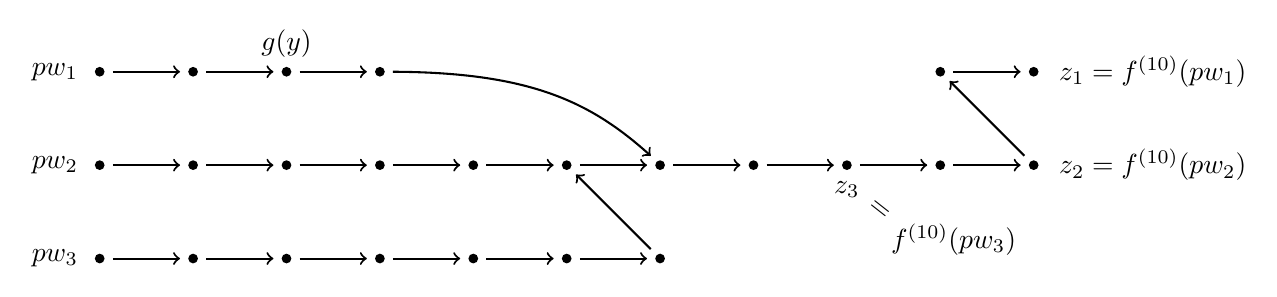
\begin{tikzpicture}[x=0.75pt,y=0.75pt,yscale=-0.9,xscale=0.9]


\draw  [fill={rgb, 255:red, 0; green, 0; blue, 0 }  ,fill opacity=1 ] (38,30) .. controls (38,28.9) and (38.9,28) .. (40,28) .. controls (41.1,28) and (42,28.9) .. (42,30) .. controls (42,31.1) and (41.1,32) .. (40,32) .. controls (38.9,32) and (38,31.1) .. (38,30) -- cycle ;
\draw  [fill={rgb, 255:red, 0; green, 0; blue, 0 }  ,fill opacity=1 ] (88,30) .. controls (88,28.9) and (88.9,28) .. (90,28) .. controls (91.1,28) and (92,28.9) .. (92,30) .. controls (92,31.1) and (91.1,32) .. (90,32) .. controls (88.9,32) and (88,31.1) .. (88,30) -- cycle ;
\draw  [fill={rgb, 255:red, 0; green, 0; blue, 0 }  ,fill opacity=1 ] (138,30) .. controls (138,28.9) and (138.9,28) .. (140,28) .. controls (141.1,28) and (142,28.9) .. (142,30) .. controls (142,31.1) and (141.1,32) .. (140,32) .. controls (138.9,32) and (138,31.1) .. (138,30) -- cycle ;
\draw  [fill={rgb, 255:red, 0; green, 0; blue, 0 }  ,fill opacity=1 ] (188,30) .. controls (188,28.9) and (188.9,28) .. (190,28) .. controls (191.1,28) and (192,28.9) .. (192,30) .. controls (192,31.1) and (191.1,32) .. (190,32) .. controls (188.9,32) and (188,31.1) .. (188,30) -- cycle ;
\draw  [fill={rgb, 255:red, 0; green, 0; blue, 0 }  ,fill opacity=1 ] (38,80) .. controls (38,78.9) and (38.9,78) .. (40,78) .. controls (41.1,78) and (42,78.9) .. (42,80) .. controls (42,81.1) and (41.1,82) .. (40,82) .. controls (38.9,82) and (38,81.1) .. (38,80) -- cycle ;
\draw  [fill={rgb, 255:red, 0; green, 0; blue, 0 }  ,fill opacity=1 ] (88,80) .. controls (88,78.9) and (88.9,78) .. (90,78) .. controls (91.1,78) and (92,78.9) .. (92,80) .. controls (92,81.1) and (91.1,82) .. (90,82) .. controls (88.9,82) and (88,81.1) .. (88,80) -- cycle ;
\draw  [fill={rgb, 255:red, 0; green, 0; blue, 0 }  ,fill opacity=1 ] (138,80) .. controls (138,78.9) and (138.9,78) .. (140,78) .. controls (141.1,78) and (142,78.9) .. (142,80) .. controls (142,81.1) and (141.1,82) .. (140,82) .. controls (138.9,82) and (138,81.1) .. (138,80) -- cycle ;
\draw  [fill={rgb, 255:red, 0; green, 0; blue, 0 }  ,fill opacity=1 ] (188,80) .. controls (188,78.9) and (188.9,78) .. (190,78) .. controls (191.1,78) and (192,78.9) .. (192,80) .. controls (192,81.1) and (191.1,82) .. (190,82) .. controls (188.9,82) and (188,81.1) .. (188,80) -- cycle ;
\draw  [fill={rgb, 255:red, 0; green, 0; blue, 0 }  ,fill opacity=1 ] (38,130) .. controls (38,128.9) and (38.9,128) .. (40,128) .. controls (41.1,128) and (42,128.9) .. (42,130) .. controls (42,131.1) and (41.1,132) .. (40,132) .. controls (38.9,132) and (38,131.1) .. (38,130) -- cycle ;
\draw  [fill={rgb, 255:red, 0; green, 0; blue, 0 }  ,fill opacity=1 ] (88,130) .. controls (88,128.9) and (88.9,128) .. (90,128) .. controls (91.1,128) and (92,128.9) .. (92,130) .. controls (92,131.1) and (91.1,132) .. (90,132) .. controls (88.9,132) and (88,131.1) .. (88,130) -- cycle ;
\draw  [fill={rgb, 255:red, 0; green, 0; blue, 0 }  ,fill opacity=1 ] (138,130) .. controls (138,128.9) and (138.9,128) .. (140,128) .. controls (141.1,128) and (142,128.9) .. (142,130) .. controls (142,131.1) and (141.1,132) .. (140,132) .. controls (138.9,132) and (138,131.1) .. (138,130) -- cycle ;
\draw  [fill={rgb, 255:red, 0; green, 0; blue, 0 }  ,fill opacity=1 ] (188,130) .. controls (188,128.9) and (188.9,128) .. (190,128) .. controls (191.1,128) and (192,128.9) .. (192,130) .. controls (192,131.1) and (191.1,132) .. (190,132) .. controls (188.9,132) and (188,131.1) .. (188,130) -- cycle ;
\draw  [fill={rgb, 255:red, 0; green, 0; blue, 0 }  ,fill opacity=1 ] (238,80) .. controls (238,78.9) and (238.9,78) .. (240,78) .. controls (241.1,78) and (242,78.9) .. (242,80) .. controls (242,81.1) and (241.1,82) .. (240,82) .. controls (238.9,82) and (238,81.1) .. (238,80) -- cycle ;
\draw  [fill={rgb, 255:red, 0; green, 0; blue, 0 }  ,fill opacity=1 ] (288,80) .. controls (288,78.9) and (288.9,78) .. (290,78) .. controls (291.1,78) and (292,78.9) .. (292,80) .. controls (292,81.1) and (291.1,82) .. (290,82) .. controls (288.9,82) and (288,81.1) .. (288,80) -- cycle ;
\draw  [fill={rgb, 255:red, 0; green, 0; blue, 0 }  ,fill opacity=1 ] (338,80) .. controls (338,78.9) and (338.9,78) .. (340,78) .. controls (341.1,78) and (342,78.9) .. (342,80) .. controls (342,81.1) and (341.1,82) .. (340,82) .. controls (338.9,82) and (338,81.1) .. (338,80) -- cycle ;
\draw  [fill={rgb, 255:red, 0; green, 0; blue, 0 }  ,fill opacity=1 ] (238,130) .. controls (238,128.9) and (238.9,128) .. (240,128) .. controls (241.1,128) and (242,128.9) .. (242,130) .. controls (242,131.1) and (241.1,132) .. (240,132) .. controls (238.9,132) and (238,131.1) .. (238,130) -- cycle ;
\draw  [fill={rgb, 255:red, 0; green, 0; blue, 0 }  ,fill opacity=1 ] (288,130) .. controls (288,128.9) and (288.9,128) .. (290,128) .. controls (291.1,128) and (292,128.9) .. (292,130) .. controls (292,131.1) and (291.1,132) .. (290,132) .. controls (288.9,132) and (288,131.1) .. (288,130) -- cycle ;
\draw  [fill={rgb, 255:red, 0; green, 0; blue, 0 }  ,fill opacity=1 ] (338,130) .. controls (338,128.9) and (338.9,128) .. (340,128) .. controls (341.1,128) and (342,128.9) .. (342,130) .. controls (342,131.1) and (341.1,132) .. (340,132) .. controls (338.9,132) and (338,131.1) .. (338,130) -- cycle ;
\draw  [fill={rgb, 255:red, 0; green, 0; blue, 0 }  ,fill opacity=1 ] (388,80) .. controls (388,78.9) and (388.9,78) .. (390,78) .. controls (391.1,78) and (392,78.9) .. (392,80) .. controls (392,81.1) and (391.1,82) .. (390,82) .. controls (388.9,82) and (388,81.1) .. (388,80) -- cycle ;
\draw  [fill={rgb, 255:red, 0; green, 0; blue, 0 }  ,fill opacity=1 ] (438,80) .. controls (438,78.9) and (438.9,78) .. (440,78) .. controls (441.1,78) and (442,78.9) .. (442,80) .. controls (442,81.1) and (441.1,82) .. (440,82) .. controls (438.9,82) and (438,81.1) .. (438,80) -- cycle ;
\draw  [fill={rgb, 255:red, 0; green, 0; blue, 0 }  ,fill opacity=1 ] (488,80) .. controls (488,78.9) and (488.9,78) .. (490,78) .. controls (491.1,78) and (492,78.9) .. (492,80) .. controls (492,81.1) and (491.1,82) .. (490,82) .. controls (488.9,82) and (488,81.1) .. (488,80) -- cycle ;
\draw  [fill={rgb, 255:red, 0; green, 0; blue, 0 }  ,fill opacity=1 ] (538,80) .. controls (538,78.9) and (538.9,78) .. (540,78) .. controls (541.1,78) and (542,78.9) .. (542,80) .. controls (542,81.1) and (541.1,82) .. (540,82) .. controls (538.9,82) and (538,81.1) .. (538,80) -- cycle ;
\draw  [fill={rgb, 255:red, 0; green, 0; blue, 0 }  ,fill opacity=1 ] (488,30) .. controls (488,28.9) and (488.9,28) .. (490,28) .. controls (491.1,28) and (492,28.9) .. (492,30) .. controls (492,31.1) and (491.1,32) .. (490,32) .. controls (488.9,32) and (488,31.1) .. (488,30) -- cycle ;
\draw  [fill={rgb, 255:red, 0; green, 0; blue, 0 }  ,fill opacity=1 ] (538,30) .. controls (538,28.9) and (538.9,28) .. (540,28) .. controls (541.1,28) and (542,28.9) .. (542,30) .. controls (542,31.1) and (541.1,32) .. (540,32) .. controls (538.9,32) and (538,31.1) .. (538,30) -- cycle ;


\draw  [->]  (47,30) -- (83,30) ;
\draw  [->]  (97,30) -- (133,30) ;
\draw  [->]  (147,30) -- (183,30) ;
\draw  [->]  (497,30) -- (533,30) ;

\draw  [->]  (47,80) -- (83,80) ;
\draw  [->]  (97,80) -- (133,80) ;
\draw  [->]  (147,80) -- (183,80) ;
\draw  [->]  (197,80) -- (233,80) ;
\draw  [->]  (247,80) -- (283,80) ;
\draw  [->]  (297,80) -- (333,80) ;
\draw  [->]  (347,80) -- (383,80) ;
\draw  [->]  (397,80) -- (433,80) ;
\draw  [->]  (447,80) -- (483,80) ;
\draw  [->]  (497,80) -- (533,80) ;

\draw  [->]  (47,130) -- (83,130) ;
\draw  [->]  (97,130) -- (133,130) ;
\draw  [->]  (147,130) -- (183,130) ;
\draw  [->]  (197,130) -- (233,130) ;
\draw  [->]  (247,130) -- (283,130) ;
\draw  [->]  (297,130) -- (333,130) ;

\draw  [->]  (335,125) -- (295,85) ;
\draw  [->]  (535,75) -- (495,35) ;

\draw  [->]  (197,30) .. controls (270.33,30.33) and (302.67,46) .. (335,75) ;

\draw (2,30) node [anchor=west] [inner sep=0.75pt]    {$pw_{1}$};
\draw (2,80) node [anchor=west] [inner sep=0.75pt]    {$pw_{2}$};
\draw (2,130) node [anchor=west] [inner sep=0.75pt]    {$pw_{3}$};
\draw (140,24) node [anchor=south] [inner sep=0.75pt]    {$g( y)$};
\draw (440,87) node [anchor=north] [inner sep=0.75pt]    {$z_{3}$};
\draw (552,30) node [anchor=west] [inner sep=0.75pt]    {$z_{1} =f^{( 10)}( pw_{1})$};
\draw (552,80) node [anchor=west] [inner sep=0.75pt]    {$z_{2} =f^{( 10)}( pw_{2})$};
\draw (462,120) node [anchor=west] [inner sep=0.75pt]    {$f^{( 10)}( pw_{3})$};
\draw (454,96) node [anchor=north west][inner sep=0.75pt]  [rotate=-38.18]  {$=$};


\end{tikzpicture}
  \caption{一个链碰撞实例,三条链的长度都是 $10$}
  \label{fig:18-14}
\end{figure}

\begin{snote}[彩虹表。]
链合并问题的一个优雅的解决方案是为图 \ref{fig:18-13-a} 的每一列 $i=1,\dots,\tau$ 使用不同的还原函数 $g_i:\mathcal{Y}\to\mathcal{P}$。和之前一样,令 $f_i(pw)= g_i(h(pw))$。预处理算法 $\mathcal{A}_0$ 现在执行图 \ref{fig:18-13-b} 中的流程。它输出一张与之前相同的表 $L$,该表包含每条链的起点和终点。如果把每条链染上不同的颜色,然后将它们略微向上弯曲,图片看起来就像是一道彩虹,这就是它名字的由来。

在每一列中使用不同的函数 $f_i$ 的意义在于,链的碰撞不一定会导致链的合并。只有当两条链在完全相同的索引处发生碰撞时,它们才会合并。这使得链合并的概率大大降低(见练习 \ref{exer:18-18})。此外,如果一条以 $pw$ 为起点的链恰好与一条以 $pw'$ 为起点的链合并,这两条链的终点 $z$ 和 $z'$ 也会是相等的。预处理算法 $\mathcal{A}_0$ 可以很容易地检测到这种重复的终点,并丢弃掉其中的一条链。最终的结果是,我们可以设定 $\tau=N^{1/3}$,$\ell=N^{2/3}$,并在预处理过程中捕获 $\mathcal{P}$ 的一个恒定比例的部分。

现在,想要用表 $L$ 计算元素 $y\in\mathcal{Y}$ 的逆,注意到,如果 $g(y)$ 包含在图 \ref{fig:18-13-b} 的倒数第二列中,$f_\tau(g(y))$ 就是 $L$ 中某条链的终点;如果 $g(y)$ 包含在图的倒数第三列中,$f_{\tau}f_{\tau-1}(g(y))$ 就是 $L$ 中某条链的终点,以此类推。这就为我们提供了下面这个使用 $L$ 计算 $y$ 的逆的算法:

\vspace*{10pt}

\hspace*{5pt} 算法 $\mathcal{A}_1(L,y)$:\\
\hspace*{26pt} 1. \quad 令 $z\leftarrow g(y)\in\mathcal{P}$\\
\hspace*{26pt} 2. \quad 对于 $i=\tau-1,\dots,0$:\\
\hspace*{26pt} 3. \quad\qquad 如果存在某个 $\widetilde{pw}$ 使得 $(\widetilde{pw},z)\in L$:
\hspace*{40pt} // \emph{如果 $z$ 是一条链的终点} \\
\hspace*{26pt} 4. \quad\qquad\qquad 令 $pw\leftarrow f_i\big(\cdots f_2(f_1(\widetilde{pw}))\cdots\big)$
\hspace*{43pt} // \emph{从起点开始遍历链} \\
\hspace*{26pt} 5. \quad\qquad\qquad 如果 $h(pw)=y$:
\hspace*{107pt} // \emph{如果发现逆元,将其输出} \\
\hspace*{116pt} 输出 $pw$ 并终止\\
\hspace*{26pt} 6. \quad\qquad 令 $z\leftarrow f_{\tau}\big(f_{\tau-1}(\cdots f_{i+1}(g(y))\cdots)\big) \in\mathcal{P}$
\hspace*{25pt} // \emph{检查 $g(y)$ 是否在第 $i$ 列上} \\
\hspace*{26pt} 7. \quad 输出 $\mathsf{fail}$
\hspace*{188.5pt} // \emph{$g(y)$ 不在任何一条链上}

\vspace*{10pt}

\noindent
该算法的大部分工作是在第 $6$ 行完成的。在第一次迭代中,该行评估了一次 $f$,在第二次迭代中评估了两次,以此类推。总的来说,第 $6$ 行导致最坏情况下的工作量是 $1+2+\cdots+\tau=\tau(\tau+1)/2\approx\tau^2/2$。因此,$\mathcal{A}_1$ 的最大运行时间是 $t:=\tau^2/2$。为了捕获大部分的 $\mathcal{P}$,我们需要 $\tau\times\ell\geq N$,而由于 $\tau=(2t)^{1/2}$,我们可得:
\[
\ell\times(2t)^{1/2}\geq N
\]
将两边同时平方,我们可得 $\ell^2\times t\geq N^2/2$,这就与式 \ref{eq:18-9} 中承诺的时空权衡一致。还需要注意的是,算法 $\mathcal{A}_1$ 最多只能对表 $L$ 进行 $\tau$ 次查找。
\end{snote}

\begin{snote}[实践中的彩虹表。]
许多流行的哈希函数的彩虹表都是现成的。它们被设计成可以与一个叫做 \textbf{RainbowCrack} 的程序配合使用。比如说,有一张大小为 460 GB 的 SHA1 彩虹表,它可以寻找字母表 \texttt{ascii-32-95} 中所有 $8$ 字符口令的原像。这个字母表包含了美国标准键盘上的所有 $95$ 个字符。该表的成功率接近97\%,而且任何人都可以免费下载它。在 GPU 上,使用该表破解一个 $8$ 字符的 SHA1 哈希口令仅需大约一个小时。
\end{snote}

\begin{snote}[扩展。]
尽管彩虹表旨在计算随机函数的逆,但 Fiat 和 Naor 的另一个算法给出了计算任意函数 $h:\mathcal{P}\to\mathcal{Y}$ 的逆的时空权衡 \cite{fiat1991rigorous}。他们的时空权衡满足 $\ell^2t\geq\lambda N^3$,这意味着,为了在 $t$ 时间内以 $1/2$ 的概率计算函数 $h$ 的逆,他们的预处理算法必须生成一张大小约为 $(\lambda N^3/t)^{1/2}$ 的表。这里,$\lambda$ 是 $h$ 的碰撞概率,定义为 $\lambda:=\Pr[h(x)=h(y)]$,其中 $x,y\overset{\rm R}\leftarrow\mathcal{P}$。当 $h$ 是一个随机函数,并且 $|\mathcal{Y}|\gg|\mathcal{P}|$ 时,我们有 $\lambda=1/N$,这就恢复了式 \ref{eq:18-9} 中的约束。
\end{snote}